\documentclass[11pt,a4paper]{article}
\usepackage[utf8]{inputenc}
\usepackage[T1]{fontenc}
\usepackage[margin=2.3cm]{geometry}
\usepackage{amsmath}
\usepackage{microtype}
\usepackage{hyperref}
\usepackage{xcolor}
\usepackage{graphicx}
\usepackage{booktabs}
\usepackage{array}
\usepackage{float}
\usepackage{caption}
\captionsetup[figure]{font=footnotesize} % matches table captions, which already inherit
                                          % \footnotesize from the tabular body
\usepackage{enumitem}
\usepackage{titlesec}
\usepackage{fancyhdr}

\graphicspath{{../outputs/inspection/figures/}{../diagrams/}}

\titleformat{\section}{\normalfont\Large\bfseries}{\thesection}{0.6em}{}
\titleformat{\subsection}{\normalfont\large\bfseries}{\thesubsection}{0.6em}{}
\titlespacing*{\section}{0pt}{1.1em}{0.5em}
\titlespacing*{\subsection}{0pt}{0.8em}{0.3em}

\pagestyle{fancy}
\fancyhf{}
\renewcommand{\headrulewidth}{0.4pt}
\lhead{\small Route Alignment: runA $\to$ runB}
\rhead{\small \thepage}
\cfoot{}

\hypersetup{
  colorlinks=true,
  linkcolor=black,
  urlcolor=blue,
  citecolor=black,
  pdftitle={Route Alignment: runA to runB},
  pdfauthor={Emery Fathan Zwageri}
}

\setlength{\parindent}{0pt}
\setlength{\parskip}{0.5em}

\begin{document}

\begin{center}
  {\LARGE\bfseries Route Alignment: runA $\to$ runB}\\[0.25em]
  {\large Phase-2 take-home --- technical report }\\[0.2em]
  \small Emery Fathan Zwageri \quad\textbullet\quad \today
\end{center}

\section{Characterising the recordings}
\label{sec:t1}

\texttt{runA}/\texttt{runB} are two recordings of the same route (cameras \texttt{cam0},
\texttt{cam5}), delivered as raw HEVC elementary streams (no container -- almost no reliable
per-file metadata) plus a sidecar \texttt{.timestamps.txt} per camera (one capture timestamp per
line, ns since epoch, loaded as \texttt{int64} throughout -- a raw epoch value exceeds
\texttt{float64}'s exact-integer range). Declared fields came from \texttt{ffprobe}/\texttt{ffmpeg}
header parsing; measured values came from forcing a full decode and from timestamp-file
arithmetic. Code: \texttt{src/routealign/\{io\_video,timestamps\}.py}; full JSON per file:
\texttt{outputs/inspection/}.

\begin{table}[H]
  \centering
  \footnotesize
  \begin{tabular}{l l r r r r r l}
    \toprule
    Run/cam & Resolution & Size (MB) & Frames (dec./lines) & Decl.\ fps & Meas.\ fps & Route (s) & Recorded (UTC) \\
    \midrule
    runA/cam0 & 1440$\times$1080 & 129.0 & 2674 / 2695 & 10.00 & 9.992 & 267.5 & 2025-02-28 06:24 \\
    runA/cam5 & 1440$\times$1080 & 121.9 & 2674 / 2695 & 10.00 & 9.992 & 267.5 & 2025-02-28 06:24 \\
    runB/cam0 & 1440$\times$1080 & 70.0  & 2622 / 2663 & 10.00 & 9.989 & 262.4 & 2024-04-13 09:12 \\
    runB/cam5 & 1440$\times$1080 & 64.0  & 2615 / 2663 & 10.00 & 9.989 & 261.7 & 2024-04-13 09:12 \\
    \bottomrule
  \end{tabular}
  \caption{Task~1 summary (full precision in \texttt{outputs/inspection/*.json}).}
  \label{tab:t1}
\end{table}

\texttt{runB} was recorded 321 days before \texttt{runA} -- two separate real-world sessions.
A first-frame check supports this: \texttt{runA} is sunny with hard shadows; \texttt{runB} is
overcast with water droplets visible on the camera housing (both cameras), consistent with rain --
a qualitative read from individual frames, not a measured statistic.

\textbf{Frame rate.} Three candidate declarations were found and tested, not taken at face value.
\emph{Kept, 10.00\,fps}: the HEVC SPS/VUI (\texttt{ffmpeg -bsf:v trace\_headers}) gives
\texttt{time\_scale/num\_units\_in\_tick=10/1}, independently matching ffprobe's
\texttt{r\_frame\_rate}. The \textbf{measured} rate, 9.992/9.989\,fps, comes from none of
these: it is $(N_{\text{decoded}}-1)/\text{span}$, span from the timestamp file. It is close to the
declared value, but that closeness is a finding, not an assumption.

\begin{figure}[H]
  \centering
  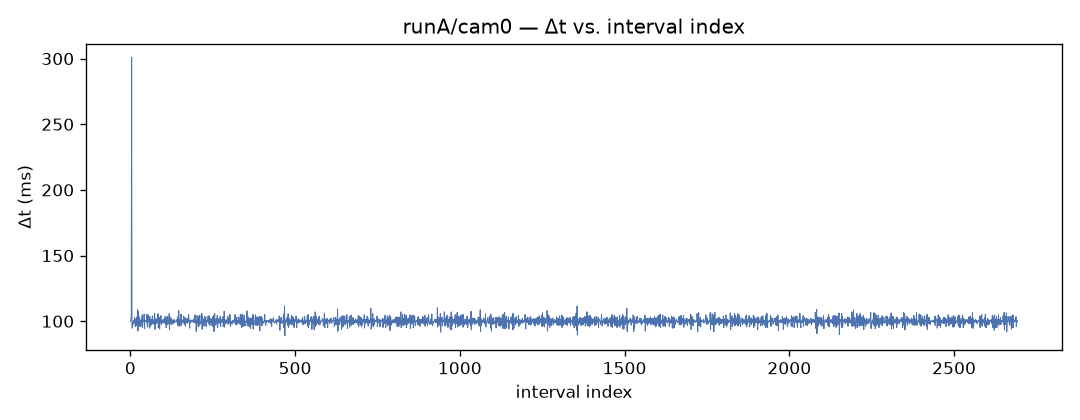
\includegraphics[width=0.72\textwidth]{runA_cam0_dt_vs_index.png}
  \caption{Interval between consecutive frames vs.\ index, \texttt{runA/cam0} (all four files show
  the same shape). A single 300.8\,ms spike (runA) / 396.9\,ms (runB) sits in the first few frames;
  the two frames bracketing each gap are visually indistinguishable, ruling out a scene event --
  most likely a one-off recording start-up cost, mechanism unconfirmed. No other file shows any
  comparable gap.}
  \label{fig:dt}
\end{figure}

\textbf{Frame-count discrepancy.} Every file has more timestamp lines than frames that actually
decode (runA: 2695 vs.\ 2674, both cameras; runB: 2663 vs.\ 2622(cam0)/2615(cam5) -- \emph{not} identical
between cameras, so the usable range must be tracked per camera). All four files are an exact
multiple of 262144\,B (256\,KiB), consistent with -- not proof of -- a writer that stopped without
a final flush; no truncation warning appears on decode either way, and no byte-level NAL scan has
confirmed an incomplete final unit. Consequence for Task~2: the mapping's H0 convention (timestamp
line $k$ = decoded frame $k$) holds only up to each file's decoded count; lines beyond it have no
video and are marked as such, never forced into a match.

\section{Matching frames between runA and runB}
\label{sec:t2}

\begin{figure}[H]
  \centering
  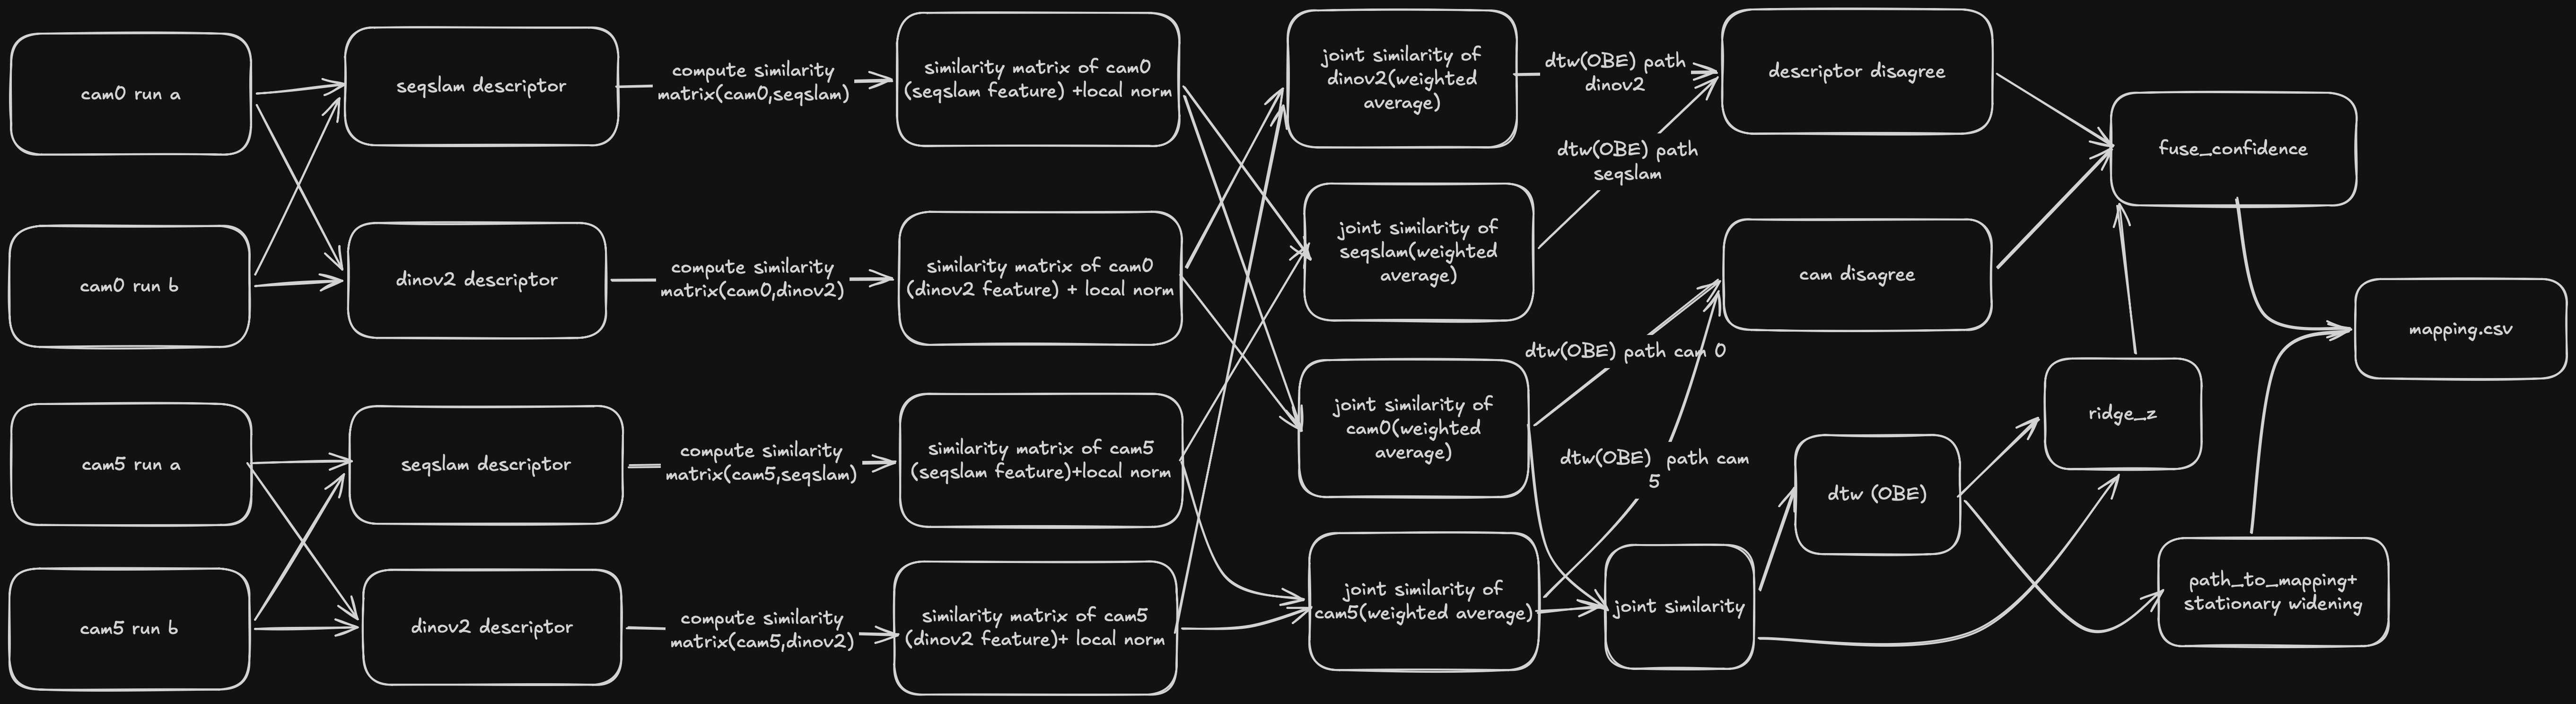
\includegraphics[width=\textwidth]{pipeline.png}
  \caption{Method pipeline, both runs $\times$ both cameras $\times$ both descriptors through to
  \texttt{mapping.csv}. Four similarity matrices (camera $\times$ descriptor) fuse two ways --
  per camera and per descriptor -- before combining into one $\hat S_{\mathrm{joint}}$;
  \texttt{dtw\_open\_ends} (``OBE'') runs on the joint matrix and, separately, on each single-axis
  matrix, so the single-axis paths can disagree with the joint one
  (\texttt{cam\_disagree}, \texttt{desc\_disagree}); \texttt{ridge\_z} from the joint path and the
  two disagreement cues feed \texttt{fuse\_confidence}.}
  \label{fig:t2-pipeline}
\end{figure}

\subsection{Method}

Four decisions, per the brief. \textbf{Representation}: two descriptors, fused rather than chosen
between -- a classical SeqSLAM-style patch-normalised grayscale descriptor (cheap,
illumination-robust) and a pretrained DINOv2 ViT-S/14 embedding (semantic, learned), each computed
per camera, per frame. \textbf{Search}: cosine similarity, then \emph{local} contrast
normalisation along each runA row (window tuned per descriptor -- 50 for SeqSLAM, 500 for DINOv2,
\S\ref{sec:ledger}), fused into one $\hat S_{\mathrm{joint}}$ by a z-scored weighted average across
both cameras and both descriptors. \textbf{Constraint}: both runs traverse the route in the same
order, so the match must be monotone -- dynamic time warping with open ends
(\texttt{dtw\_open\_ends}), never an unconstrained per-row argmax. \textbf{Confident vs.\ wrong}:
four agreement cues computed once the path is fixed -- \texttt{ridge\_z} (path strength along its
own trajectory), \texttt{margin\_z} (claimed match vs.\ the best alternative outside a
$\pm 30$-column band), \texttt{cam\_disagree} (cam0-only vs.\ cam5-only path),
\texttt{desc\_disagree} (SeqSLAM-only vs.\ DINOv2-only path) -- fused into an ordinal 4-tier
confidence plus an explicit no-match rule (\texttt{runB\_frame} left empty). Concretely:
\textbf{0.9} requires \texttt{ridge\_z} $\geq 1.5$ with both disagreements $\leq 3$ frames;
\textbf{0.7} requires \texttt{ridge\_z} $\geq 1.0$ with both disagreements $\leq 5$; \textbf{0.5}
marks rows whose match is a stationary plateau (a range, not one frame); everything else that
survives stays at \textbf{0.4} -- matched, but clearing no tier's bar. No-match fires on
\texttt{ridge\_z} $< \tau = 0.75$ ($\tau$ from a synthetic deletion test, not a guess), on a
boundary-clamped row with \texttt{ridge\_z} $< 1.5$, or on both disagreements $> 30$. The tiers
are an ordinal ranking whose meaning is \emph{measured} (the reliability table,
Table~\ref{tab:reliability}), not a calibrated probability.

\textbf{Alternatives considered}: a single descriptor was
rejected -- SeqSLAM alone is cheap but collapses under rain/low-texture stretches, DINOv2 alone
has no classical baseline to cross-check against; early fusion (concatenating descriptors before
similarity) was tested for real (\S\ref{sec:t2-ablation}), not just argued about.

\subsection{Results}

\texttt{outputs/mapping.csv}: 2695 rows, one per runA timestamp line. \texttt{status}: matched
2488, ambiguous\_range 124 (inside a stop/plateau -- real match, not frame-exact), no\_match 62
(abstained), no\_frame 21 (H0 tail, no decoded frame at all). Confidence tiers: 0.9 (926 rows),
0.7 (1104), 0.5 (24), 0.4 (558).

\begin{table}[H]
  \centering\footnotesize
  \begin{tabular}{lrrr}
    \toprule
    Confidence tier & $n$ (scored anchors) & correct & measured accuracy \\
    \midrule
    0.9 & 8 & 8 & 100\% \\
    0.7 & 7 & 5 & 71\% \\
    0.4 & 4 & 2 & 50\% \\
    \bottomrule
  \end{tabular}
  \caption{Reliability table: measured accuracy per confidence tier, against 19 user-verified
  anchors. Monotonic -- confidence is an honest ordinal ranking, not just a number.}
  \label{tab:reliability}
\end{table}

\subsection{Ablation}
\label{sec:t2-ablation}

\begin{table}[H]
  \centering\footnotesize
  \setlength{\tabcolsep}{4.5pt}
  \begin{tabular}{l rrr rr rrr}
    \toprule
    & \multicolumn{3}{c}{position error (20 anchors)} & \multicolumn{2}{c}{pred.\ at no-GT}
    & \multicolumn{3}{c}{\texttt{ridge\_z}-only gate} \\
    \cmidrule(lr){2-4}\cmidrule(lr){5-6}\cmidrule(lr){7-9}
    Configuration & median & p90 & hit@5 & @2600 & @2650 & f.-abst. & z@2600 & z@2650 \\
    \midrule
    argmax on $S_{\mathrm{joint}}$ (no DTW) & 0.0 & 556.3 & 0.65 & 655 & 655 & 0/20 & 1.59 & 1.47 \\
    SeqSLAM only, late fusion & 0.0 & 79.2 & 0.85 & 2597 & 2600 & 1/20 & \textbf{0.36} & 1.17 \\
    SeqSLAM only, early fusion & 0.0 & 3.7 & 0.90 & 2598 & 2600 & 0/20 & 0.90 & 1.46 \\
    DINOv2 only, late fusion & 0.0 & 4.3 & 0.90 & 2606 & 2614 & 1/20 & \textbf{0.56} & 0.78 \\
    DINOv2 only, early fusion & 0.0 & 4.1 & 0.90 & 2604 & 2614 & 0/20 & \textbf{0.46} & 0.79 \\
    All-4 early fusion (concat) & 0.0 & 3.5 & 0.90 & 2597 & 2600 & 0/20 & \textbf{0.39} & 1.02 \\
    cam0 only (both descriptors) & 0.0 & 3.7 & 0.90 & 2600 & 2600 & 0/20 & 0.75 & 1.31 \\
    cam5 only (both descriptors) & \textbf{2.0} & 7.9 & 0.85 & 2585 & 2587 & 2/20 & 0.94 & 0.90 \\
    \textbf{Joint late fusion -- shipped} & 0.0 & \textbf{3.5} & 0.90 & 2597 & 2600 & 1/20 & \textbf{0.36} & 0.79 \\
    \bottomrule
  \end{tabular}
  \caption{Ablation, one row per configuration (early/late fusion = descriptor concatenation
  vs.\ score averaging). \emph{Left}: position error in frames against the 20 of 22 anchors
  that have a ground-truth position -- the other 2 (2600, 2650) are genuine loop-closure
  no-matches with no position to score (\S\ref{sec:t2-groundtruth}). \emph{Middle}: the raw DTW
  candidate at those 2 anchors -- a bare path cannot output ``no match'', it always returns some
  column. \emph{Right}: a \texttt{ridge\_z}-only no-match gate, same $\tau=0.75$/window 5 as the
  shipped pipeline but without \texttt{cam\_disagree}/\texttt{desc\_disagree} (most
  configurations have no second, independently-computed path to disagree with); f.-abst.\ = how
  many of the 20 real-position anchors it would wrongly abstain on. Bold ridge = caught
  ($<\tau$); bold elsewhere = the notable value in its column.}
  \label{tab:ablation}
\end{table}

Four findings worth defending individually. \textbf{DTW is doing real work}: p90 556.3 $\to$ 3.5
frames once monotonicity is added -- the quantitative version of Fig.~\ref{fig:t2-argmax}'s corner
aliasing. \textbf{cam5 is measurably worse}: median 2.0 vs.\ 0.0, p90 7.9 vs.\ 3.7 -- cam5
(road-facing) sees more passing traffic than cam0 (kerb-facing), confirmed visually in
Fig.~\ref{fig:failures}. \textbf{Early vs.\ late camera fusion, tested not argued}: SeqSLAM
benefits hugely from early fusion (79.2 $\to$ 3.7 -- late fusion's score averaging lets one
camera's false attractor dominate; concatenation needs \emph{joint} agreement first); DINOv2
barely changes (4.3 $\to$ 4.1). Shipped late-fusion still matches early fusion's best result
(3.5 vs.\ 3.7) through a different mechanism (descriptor, not camera, redundancy) while keeping
\texttt{cam\_disagree}/\texttt{desc\_disagree} computable, which full early fusion would preclude.
\textbf{Recognising ``no match'' is hard for every configuration}: at the 2 no-GT anchors all
8 DTW rows agree on \emph{where} to within 29 frames of each other (argmax's 655/655 is
Fig.~\ref{fig:t2-argmax}'s corner aliasing again -- two rows 50 apart collapsing onto one wrong
attractor column); the ridge-only gate catches 2650 for none of the 9 and 2600 for five. The
shipped \texttt{fuse\_confidence} correctly suppresses 2600 (\texttt{ridge\_z}=0.36) but lets
2650 through at confidence 0.4 (\texttt{ridge\_z}=0.79 $\geq\tau$), and its one false abstain
(anchor 183, \texttt{ridge\_z}=0.69) is identical with or without the disagreement cues,
cross-checked against \texttt{outputs/evaluation\_anchors.csv} -- on this sample those cues
changed no abstain decision; their contribution is the reliability table's tier separation, not
the no-match rule.

\begin{figure}[H]
  \centering
  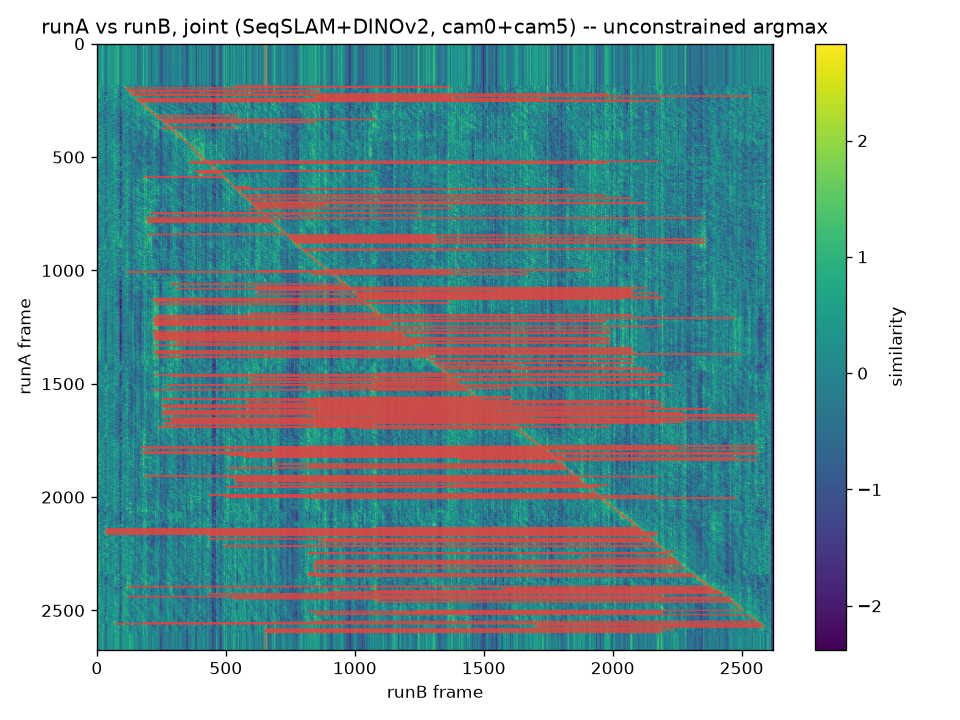
\includegraphics[width=0.46\textwidth]{step3_similarity_argmax_diagnostic.png}
  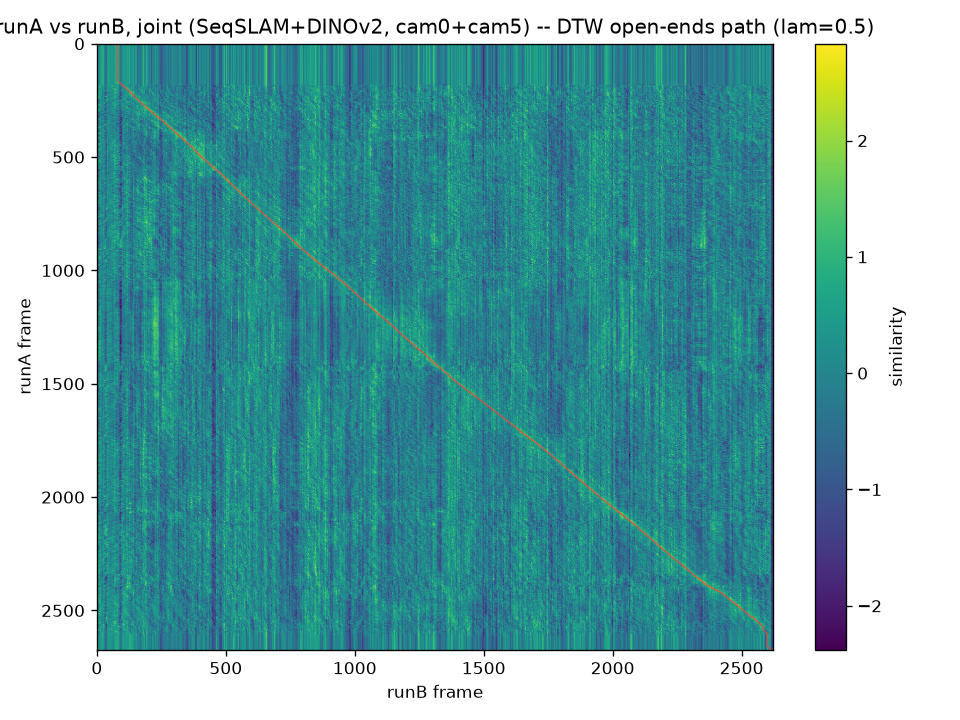
\includegraphics[width=0.46\textwidth]{step4_dtw_path_diagnostic.png}
  \caption{Unconstrained per-row argmax (left) aliases onto visually similar but wrong columns;
  DTW with the monotonicity constraint (right) tracks the true diagonal.}
  \label{fig:t2-argmax}
\end{figure}

\subsection{Ground truth and an honest accuracy estimate}
\label{sec:t2-groundtruth}

22 stratum-S anchors (runA 200--2500 roughly every 115 frames, plus the plateau at 60/150 and the
loop-closure tail at 2600/2650), labelled by a human from model-blind browsing sheets
(\texttt{gt-sheets}) against a fixed protocol (\texttt{gt/labelling\_protocol.md}: same place =
within $\pm 0.5$\,s of runB travel, lane offset ignored) -- never used for tuning. 19 of 22 have a
position to score (3 are \texttt{no\_match} on one side or the other, see below).
\textbf{median error 0.0 frames, p90 4.2 frames, hit@2/5/10 89.5\%}, Wilson 95\% CI on hit@5
$[68.6\%, 97.1\%]$ -- quoted because $n=19$ is small enough that the interval, not just the point
estimate, is the honest number to defend. A dev/test split (6/16, as originally planned) was
considered and \textbf{deliberately not done}: splitting 22 further leaves too few anchors on
either side for a usable interval, and the deletion test (recall 1.0, precision 0.56 on a
synthetic runB deletion) already covers what the split was for -- threshold sanity, not a second
accuracy number.

\textbf{The 3 unscored anchors are informative, not discarded.} Anchor 183: ground truth
$[102,104]$, pipeline's own raw candidate (column 100) missed by only 2 frames but abstained
anyway -- \texttt{ridge\_z}=0.69 fell 0.06 short of $\tau=0.75$. Anchor 2600: correctly abstained,
\texttt{ridge\_z}=0.36, \texttt{cam\_disagree}=15.0 (both cameras genuinely disagree). Anchor 2650:
\texttt{ridge\_z}=0.79 passed $\tau$ but ground truth is a genuine loop-closure \texttt{no\_match}
-- a wrong guess let through just above the line. Net read: $\tau=0.75$ is not free of cost in
either direction at this sample size, and 3 points is descriptive, not a basis for retuning it.

\subsection{Failure cases}
\label{sec:failures}

\begin{figure}[tbp]
  \centering
  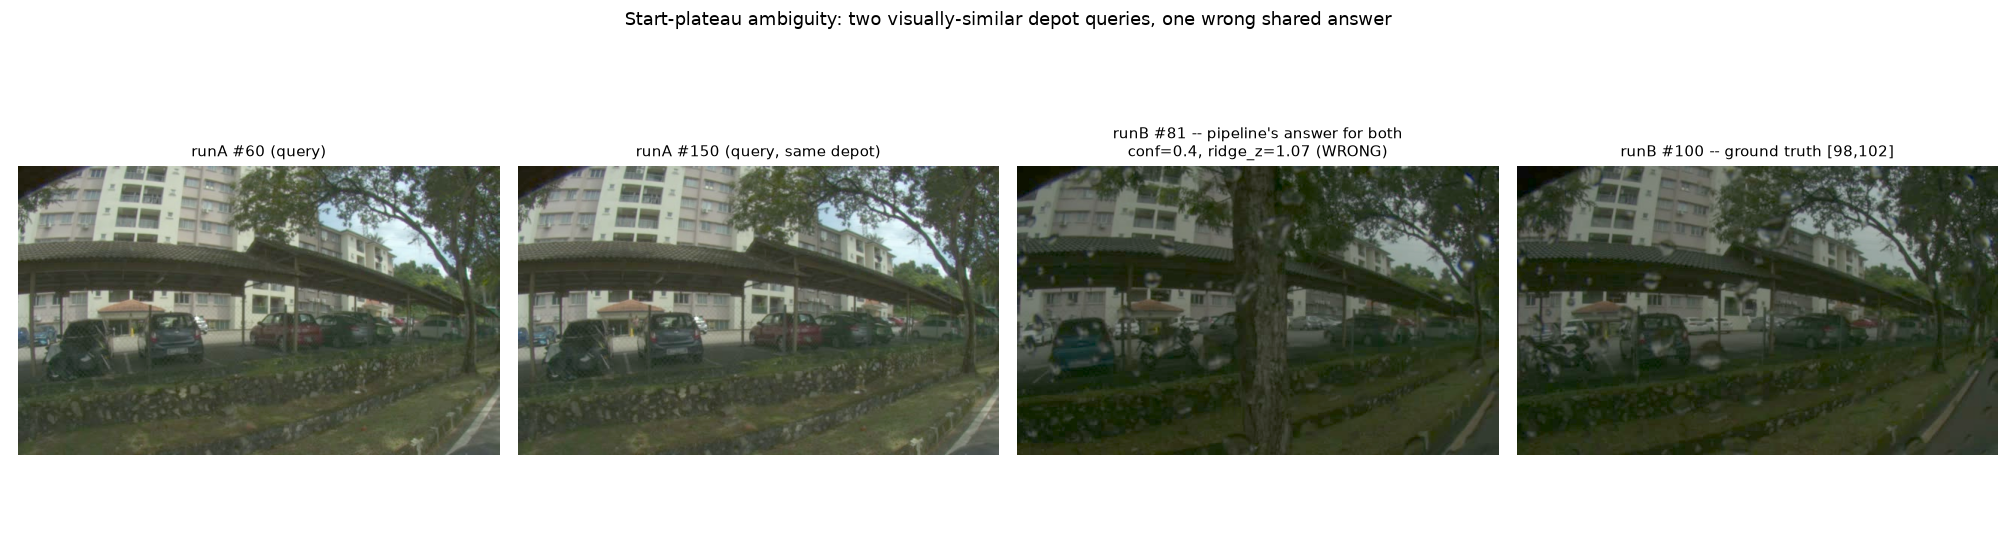
\includegraphics[width=0.48\textwidth]{failure_start_plateau.png}\hfill
  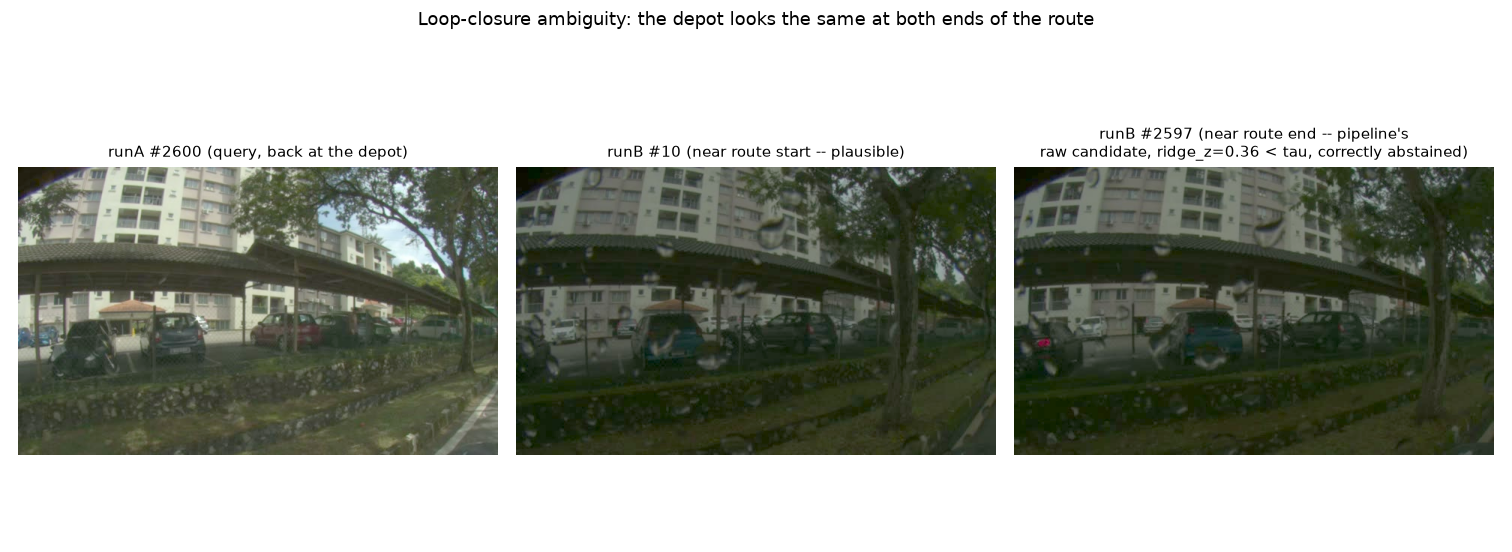
\includegraphics[width=0.48\textwidth]{failure_loop_closure.png}\\[0.4em]
  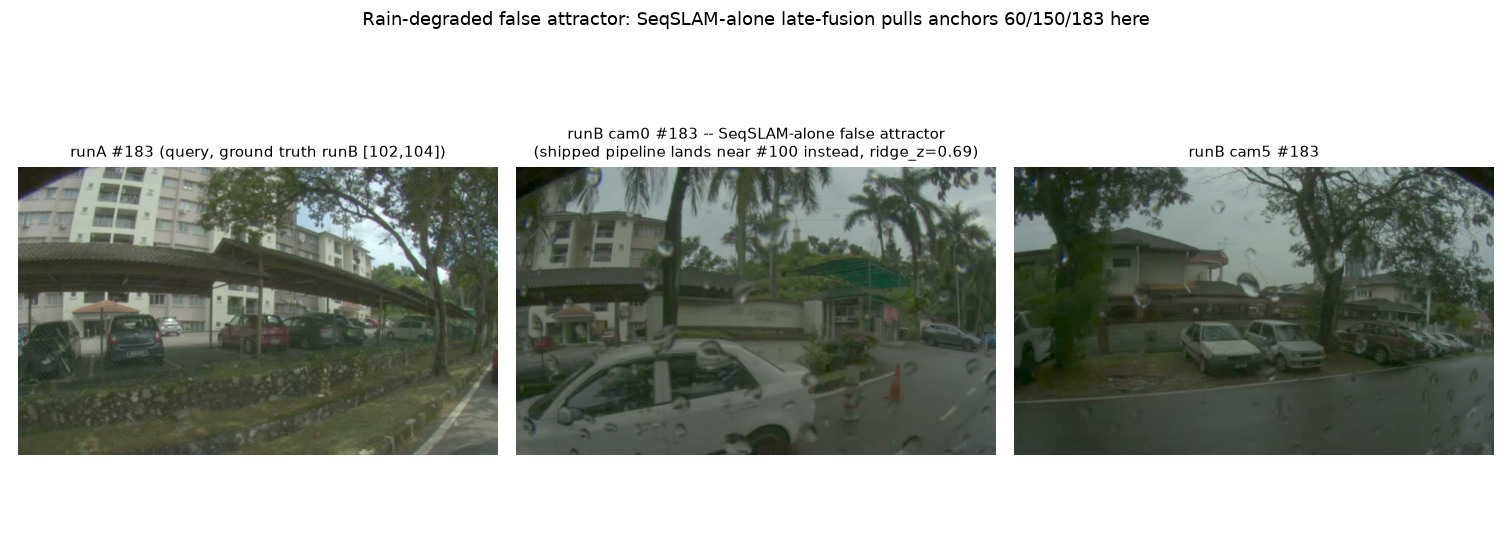
\includegraphics[width=0.48\textwidth]{failure_rain_attractor.png}\hfill
  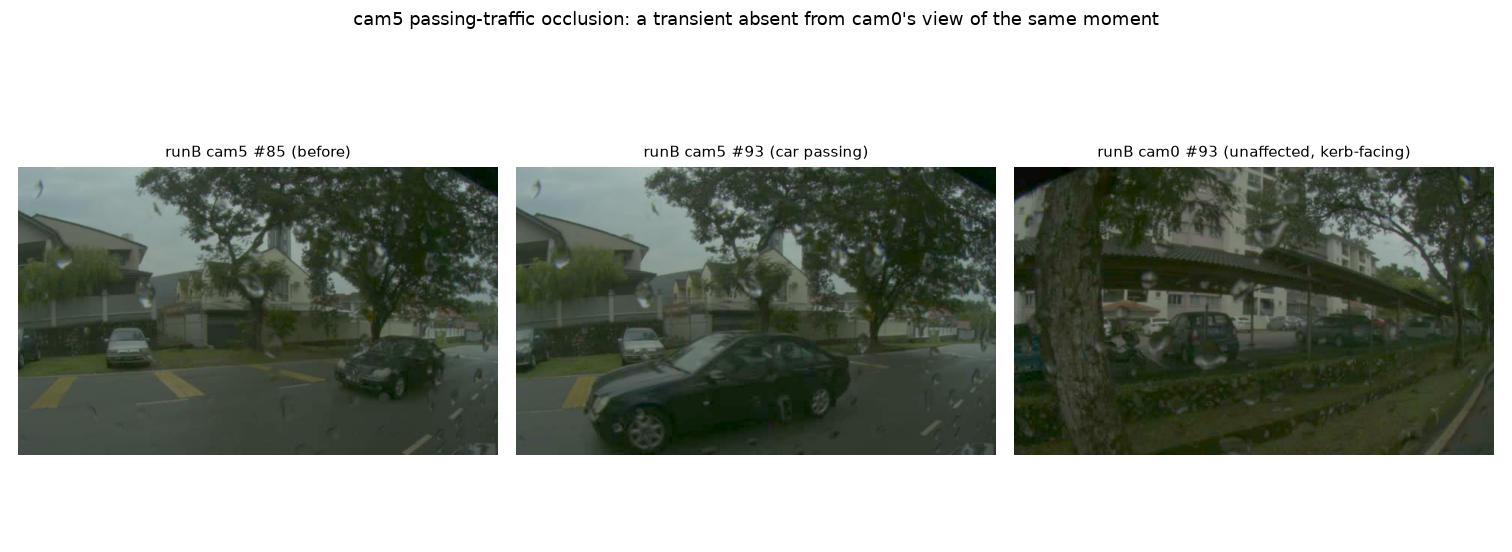
\includegraphics[width=0.48\textwidth]{failure_cam5_traffic.png}\\[0.4em]
  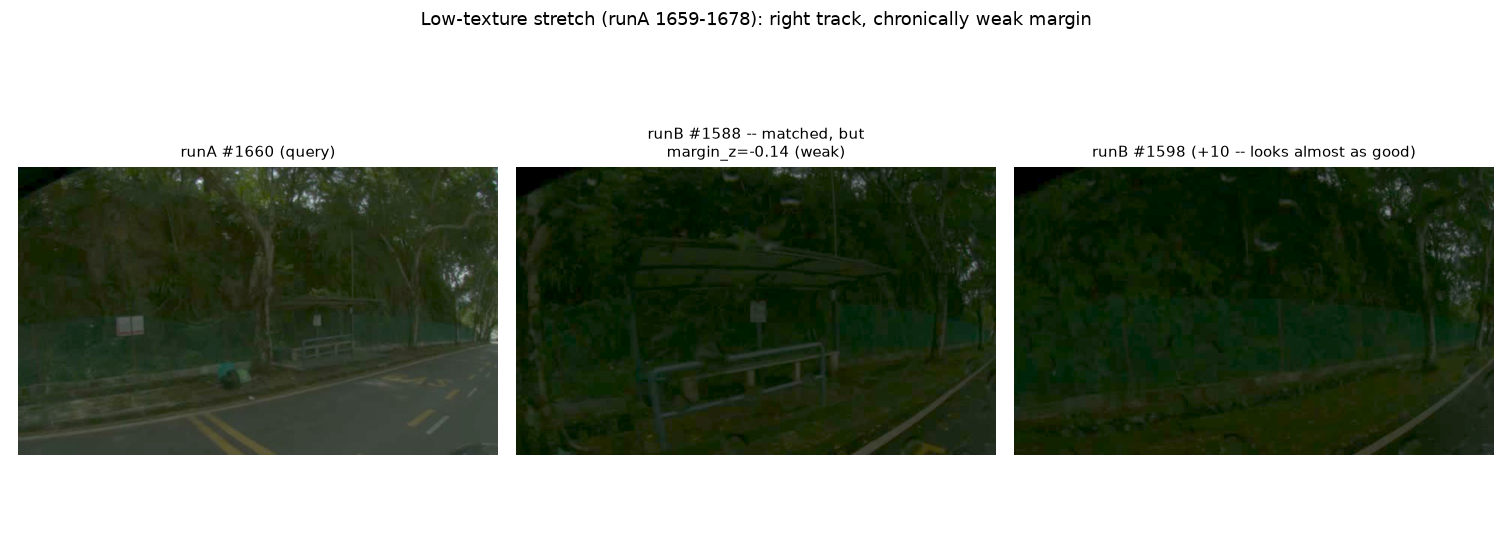
\includegraphics[width=0.48\textwidth]{failure_low_texture.png}
  \caption{Five real failure modes. \emph{Top left}: identical depot frames (runA 60, 150)
  collapse onto the same confident-wrong answer. \emph{Top right}: loop closure -- runB \#10 and
  \#2597 are nearly the same photo, so abstaining is correct. \emph{Middle left}: the rain-degraded
  scene (runB \#183) SeqSLAM's late fusion collapses onto for three anchors. \emph{Middle right}:
  a passing car occludes cam5 (motion energy peaks then drops) but not cam0 at the same index.
  \emph{Bottom}: dense canopy (runA 1659--1678) tracks correctly but with chronically negative
  \texttt{margin\_z} -- weak discrimination, not one wrong attractor.}
  \label{fig:failures}
\end{figure}

One anticipated failure mode was checked for and \textbf{not found}: "runA tail beyond runB's
truncated end" (\texttt{boundary\_clamped}). Zero rows have it set in the shipped mapping -- the
two runs' route coverage happens to reach both open ends. Reporting this honestly is worth more
than forcing an example that does not occur.

\textbf{Where the mapping is least reliable}: the depot/carport area (anchors 60, 150 -- a
visually-repetitive plateau where many runA frames are near-identical), the loop-closure tail
(2600--2673, genuinely ambiguous by construction), and any stretch under dense tree canopy (weak
margin, not wrong per se, but low-confidence by design). cam5-only performance is measurably worse
than cam0-only throughout, consistent with its greater exposure to transient occlusion.

\section{Keep/discard policy}
\label{sec:t3}

\texttt{outputs/keep\_manifest.csv}: one row per \texttt{(run, cam, frame)} -- not per timestamp
line -- because decode status, occlusion and motion genuinely differ per camera even at the same
index. $2695{\times}2 + 2663{\times}2 = 10716$ rows. \textbf{keep=10585, discard=131} -- 131 exactly
reproduces the independently-measured \texttt{no\_frame} gap (21+21+41+48), a real cross-check, not a
coincidence.

Only one rule is a hard discard: no decoded frame. Every other rule attaches a column a downstream
consumer filters on explicitly, deliberately \textbf{flag-heavy rather than discard-heavy} -- a
stationary frame is redundant for training diversity but might be exactly what a "does the model
recognise a parked scene" eval wants; discarding it pre-emptively answers a question we were not
asked. Attached per surviving frame: timing confidence (\texttt{ts\_confidence}, tail-zone flag),
interval regularity, stationary-run membership and a 1\,Hz dedup flag, run/camera-level weather,
lighting and occlusion tags, Task 2's correspondence (\texttt{corr\_*}, \texttt{"not\_applicable"}
for runB rows -- a reverse mapping was never computed or evaluated, so it is not invented here),
and a \texttt{place\_id} for split-leakage-safe train/val/test assignment (contiguous 70/15/15
blocks over $\lfloor \text{runB\_frame}/100\rfloor$, both runs' frames of one place always sharing
a split, the shared start/end depot merged into one id and left \texttt{unassigned}).

\textbf{Corrupt decode and exact duplicates -- checked, not assumed}: \texttt{motion\_energy} read
exactly 0.0 for zero consecutive-frame pairs across all 4 streams; re-decoding all 4 streams at a
stricter ffmpeg verbosity than production (\texttt{-v warning} vs.\ \texttt{-v error}) produced
zero warning lines. \texttt{keep=decode\_ok} is evidence-backed as complete for this dataset, not
merely the only rule that happened to get built.

\section{Reproducibility and the proved-vs-assumed ledger}
\label{sec:ledger}

Full reproduction steps, pinned/measured dependency versions and the \texttt{ffmpeg} build string
are in \texttt{README.md}; every number in this report was read directly from the pipeline's own
regeneratable outputs (\texttt{outputs/mapping.csv}, \texttt{outputs/keep\_manifest.csv},
\texttt{outputs/evaluation\_summary.json}, \texttt{notebooks/results/}), not transcribed from
memory. \texttt{make all} twice produces byte-identical CSVs (fixed seeds, sorted iteration, no
wall-clock values in any output).

\begin{table}[H]
  \centering\footnotesize
  \begin{tabular}{p{0.29\textwidth}p{0.14\textwidth}p{0.42\textwidth}}
    \toprule
    Claim & Status & Evidence \\
    \midrule
    H0 (frame $k$ = ts.\ line $k$ = decoded frame $k$) & \textbf{assumed}
      & GOP/IDR positions match exactly across all 4 streams for their whole usable range; no
      hardware timestamp cross-check exists \\
    Declared 10 / measured 9.99\,fps & proved & VUI matches ffprobe; measured is
      $(N_{\mathrm{decoded}}{-}1)/\mathrm{span}$ from timestamps -- independent sources \\
    Reliability table monotonicity & measured & $n=4/7/8$ per tier -- real, not
      cherry-picked, but too small to detect a mild mis-calibration \\
    No corrupt/duplicate frames & proved & zero warnings at stricter verbosity; zero
      exact-zero \texttt{motion\_energy} transitions \\
    \texttt{depot\_runb\_margin}, split 70/15/15 & \textbf{chosen} & a defensible
      convention, not the one correct policy \\
    Weather / lighting / \texttt{lens\_occlusion} & \textbf{assumed} & one-time
      visual read per run/camera, not a per-frame detector \\
    \bottomrule
  \end{tabular}
  \caption{Every claim in this report that is not a direct, repeatable measurement.}
  \label{tab:ledger}
\end{table}

\end{document}
